\chapter{Introducción}

Este documento propone y recoge el desarrollo de un proyecto de tésis que surge de la evaluación del estado actual de la robótica. En un punto en el que el despegue del sector ya ha comenzado, empieza a ser necesario atender las necesidades paralelas que surgen a su paso. Se llevó a cabo un exhaustivo estudio que trató de precisar cuáles eran estas necesidades y, sobre todo, cuáles de  ellas tenían al mismo tiempo mayor importancia y mayor valor contributivo para perpetuar el camino de la robótica. Se llegó a una única conclusión que motivó el planteamiento de la idea que aquí se detalla, la cual si bien es difícil de resumir en una frase, hemos decidido bautizar como ``hacer la robótica más accesible''.

Se buscará detallar de la manera más fiel posible el completo proceso de estudio y análisis de herramientas de naturaleza variada relacionadas con el desarrollo e implementación de aplicaciones asociadas al sector robótico y automático, el método y los criterios de selección que llevaron a la elección de unos agentes frente a otros y su conveniente combinación para la construcción de una herramienta, que creemos novedosa, que puede dar solución a una de las lagunas más visibles en lo que a docencia, aprendizaje e investigación se refiere: {\bf{su accesibilidad}}. Se tratará de evaluar la validez de la idea que se propone y su viabilidad en forma de reseña crítica a través de la implementación de la lógica e infraestructura que permita cumplir el propósito, o al menos acercarse a él, y de la evaluación de los resultados que se obtenga de su empleo. En este primer capítulo se expone tanto el contexto en el cual se sitúa este proyecto como el motivo por el cual su desarrollo puede suponer un pasó más hacia la satisfacción de una necesidad social.

\section{Robótica}

Aunque el origen de la robótica se remonta a los principios de la década de los 50, es en los últimos años cuando ha incrementado exponencialmente la presencia de estos sistemas electromecánicos en la vida cotidiana, además de en el ámbito laboral, para enfrentar problemas que resultan tediosos, repetitivos e incluso peligrosos para las personas, a la par que reducen en gran medida la carga de trabajo a la que están sometidas. Hoy en día no solamente nos rodean los robots industriales, como los presentes en líneas de producción o los involucrados en cadenas de envasado entre otros, sino que los robots adquieren cada vez mayor protagonismo y presencia en entornos alternativos, como el doméstico, militar, o el agrícola (Fig. \ref{robots}), incluso dando pie a la creación de numerosas y nuevas aplicaciones para los que son idóneos como las tareas relacionadas con logística de almacenes y envíos de mercancía o exploración espacial.

\begin{figure}[!hbtp]  \centering\noindent
    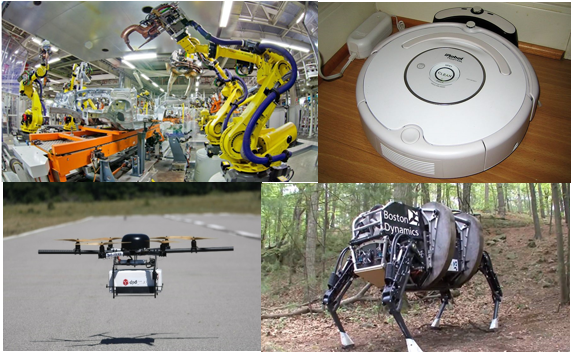
\includegraphics[width=0.7\textwidth]{figures/robots.png}
    \caption{Aplicaciones actuales de los robots.}
    \label{robots}
\end{figure}

Con el paso de los años se observa una clara tendencia hacia el diseño de sistemas robotizados para cubrir necesidades o desempeñar tareas que nunca se imaginaron automáticas. Surge, con ello, una necesidad social que requiere la instrucción de nuevos profesionales y expertos en esta potente rama de la ciencia y la tecnología que puedan lidiar con el diseño y desarrollo de estas entidades mecánicas cuyo comportamiento se espera que sea cada vez más complejo y completo, ayudando a los seres humanos no sólo a reducir costos, sino también a simplificar tareas, optimizar recursos y contribuir en labores de investigación. Es por eso que aumentan considerablemente aún hoy las ramas de estudio asociadas a la Ingeniería Automática, Mecánica, Electrónica y de Telecomunicaciones principalmente, que persiguen precisamente cubrir esa exigencia de formación para abordar un futuro lleno de robots, a la par que contribuyen a la generación de investigadores y proyectos que propulsarán el desarrollo de este sector en búsqueda del beneficio social. 

Las circunstancias idóneas para la instrucción e investigación necesario para el estudio de la Robótica no resultan sencillas de conseguir. Como ya se ha dicho, nuestro entorno actual engloba robots en grandes cantidades, pero también es cierto que el acceso a los mismos está muy restringido a cierto sector social. No se trata de un problema económico en cuanto a su adquisición, pues poco a poco el precio de producción de sistemas robóticos se reduce gracias al abaratamiento de componentes electrónicos y materiales con los que se elaboran, además de la optimización de los procesos de construcción y ensamblado de los mismos, que hacen que el precio final de los robots sea, en cierta medida, asequible para el consumidor medio dependiendo siempre de la aplicación. El problema reside más bien en que las circunstancias y los entornos de desarrollo, investigación, docencia e instrucción en la robótica son a la vez difícilmente accesibles, escasos, enormemente controlados y por último, pero quizá más importante, económicamente exigentes. Es por eso que resulta complicado el proceso de instrucción en robótica. Jamás pediríamos al escultor que aprendiera a esculpir sin cincel, o al biólogo que estudiase la naturaleza en su sótano. Sin embargo, debido al bajo grado de accesibilidad de los entornos docentes y de investigación en el campo de la robótica, en muchas ocasiones se priva de su principal herramienta de aprendizaje a los estudiantes e investigadores del campo, o se complica en gran medida su curva de entrada. En base a mi experiencia reciente puedo decir que el énfasis se pone, inevitablemente, ``sobre el papel'' en lugar de ``en la masa''.

Destaca también la carencia o escasez de entornos de aprendizaje graduales como los existentes en otros ámbitos, donde se comienza por un nivel básico que poco a poco se va incrementando. La robótica requiere, por definición, de entornos de aprendizaje e investigación altamente especializados, donde el usuario debe conocer de antemano no sólo los fundamentos básicos de los sistemas robotizados, sino también las nociones necesarias de matemáticas, física, mecánica y electrónica como mínimo, pudiendo extenderse el repertorio según el área de especialización dentro del campo.

Quedan de manifiesto las dificultades a las que se enfrenta todo aquel que quiere tener relación con la robótica.

\section{Tecnologías Web}

El crecimiento exponencial al que está sujeta la Web en los últimos tiempos hace que se vaya constituyendo un entorno ideal para el desarrollo de nuevas aplicaciones en lo relacionado con el ocio, los servicios y las necesidades de las personas. De entre los nuevos productos web más influyentes podemos encontrar ejemplos como Netflix, un servicio de video bajo demanda (VoD) que ofrece películas y series en \textit{streaming} a través de la web, o Spotify, de características similares en el caso del contenido musical, e incluso servicios de computación en la nube como Amazon Web Services sobre los que se puede construir cantidad de potentes plataformas que sirven a las personas a través de Internet como Dropbox, HootSuite o Foursqare.

Algunos años atrás resultaba impensable plantear un desarrollo robótico empleando este tipo de tecnología dado que los motores web apenas tenían potencia de cómputo suficiente para reproducir un vídeo, y mucho menos podían si quiera superar los límites del navegador para acceder a dispositivos externos. Las nuevas aplicaciones de las tecnologías web han demostrado que esta circunstancia ha cambiado hasta tal punto en que se pueden crear aplicaciones tan exigentes como juegos en realidad virtual, procesamiento de imágenes, la comúnmente llamada ``minería de datos'' o KDD e incluso tareas de aprendizaje automático gracias, entre otras cosas, a la posibilidad de acceder al \textit{hardware} de aceleración gráfica por parte del navegador y a la incorporación en el mismo de potentes núcleos o motores de ejecución, dando lugar a las aplicaciones dinámicas en la nube (Fig. \ref{web}).

\begin{figure}[!hbtp]  \centering\noindent
    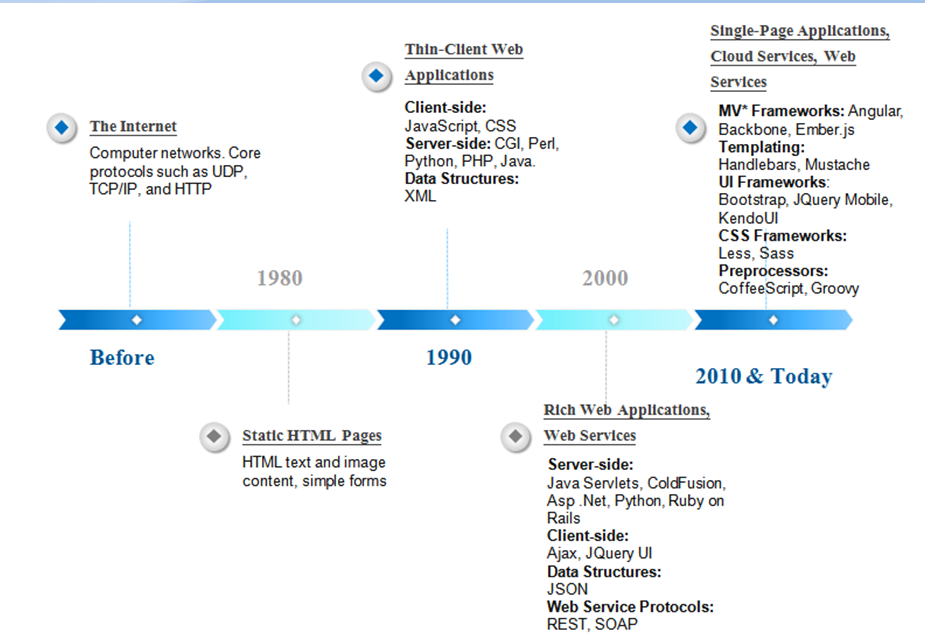
\includegraphics[width=0.99\textwidth]{figures/web-history.png}
    \caption{Evolución de las Tecnologías Web}
    \label{web}
\end{figure}

En la actualidad, se puede construir aplicaciones para casi cualquier caso de uso, incluido el de la robótica, completamente formados por herramientas web. Gran parte de sus ventajas residen en que el acceso a la web es totalmente público y sencillo, de tal manera que un servicio ofrecido a través de la web puede ser usado por cualquier persona del planeta, con independencia de su sistema operativo, dispositivo o entorno. 

Dado que Internet no es más que un conjunto debidamente interconectado de sistemas y redes de sistemas que se comunican a través de protocolos conocidos (mirándose con un gran nivel de abstracción), se puede conseguir de manera bastante eficaz conectar herramientas de distinta naturaleza para que funcionen como un conjunto homogéneo a través de Internet. Entre las funciones interconectables que nos ofrece la web, destacamos especialmente el acceso al \textit{hardware} del equipo cliente, el soporte de almacenamiento en la nube, los mecanismos de seguridad, las características de sus canales de comunicación (baja latencia punto a punto, retransmisiones, baja tasa de error y de paquetes perdidos,...) y la capacidad de ejecutar el código de la aplicación. 

Aún con todas las ventajas ya mencionadas, la característica responsable del éxito de las aplicaciones web es probablemente la facilidad de acceso que, como ya se ha dicho, se realiza a través de un navegador web. Este es el agente que tiene visibilidad tanto interna como externa, es decir, que puede comunicarse tanto con el PC o sistema en el que está instalado como con el resto del mundo, y funciona con independencia del sistema latente bajo él. Esto quiere decir que cualquier ente conectado a Internet puede acceder a las aplicaciones web, sin importar cuál sea su sistema. 

\section{Robótica a través de las Tecnologías Web}

La intersección entre el campo de la robótica y las herramientas web dispone un entorno con un gran potencial para el desarrollo de aplicaciones que permitan enfrentarse a tareas de investigación y aprendizaje con características muy atractivas.

\begin{figure}[!hbtp]  \centering\noindent
    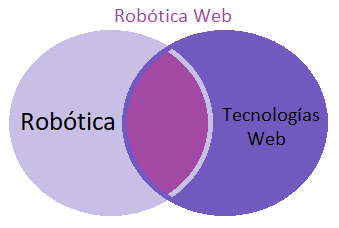
\includegraphics[width=0.55\textwidth]{figures/intersection.png}
    \caption{Entorno Robótico en la Web}
    \label{web}
\end{figure}

Investigando el panorama docente y de experimentación moderno en cuanto a robótica se refiere, encontramos numerosas librerías que ya facilitan en gran medida el trabajo con robots, como pueden ser OpenCV para tareas de Visión Artificial u OMPL para planificación de rutas, y también entornos de desarrollo y \textit{frameworks} que simplifican el proceso como ROS o YARP. 
Sin embargo, aún no se han desarrollado herramientas maduras que engloben estas nuevas tecnologías en una sola para que el trabajo con sistemas robóticos sea casi tan fácil como pulsar un botón y ver el código en acción. Hasta el momento, es necesario disponer de numerosos módulos inteligentes cuidadosamente interconectados que sincronicen y supervisen la ejecución de diferentes aspectos para lograr controlar cualquier aspecto de un robot, todos ellos necesariamente ideados y construidos por el sujeto que trata de desarrollar algo.

Aún no existen plataformas de uso extendido o estándar ``\textit{de facto}'' que permitan una buena instrucción en este joven campo de la ingeniería, siendo en muchos casos debido a que resulta muy difícil acceder a \textit{hardware} adecuado para el aprendizaje o investigación por temas económicos o restricciones externas, o llevar los conocimientos teóricos a un entorno práctico para asentar los conocimientos. Analizando el estado actual se ha encontrado algunas plataformas que ya buscan una primera aproximación hacia esa aplicación de propósito general en docencia e investigación, que tratan de disponer de todo lo necesario para que sentarse a programar un robot, o varios, resulte incluso sencillo, a la par que instructivo y alentador. Algunos ejemplos son:

\begin{itemize}

\item [$\rightarrow$] La herramienta \textit{Colaboratory}\footnote{\url{https://colab.research.google.com/notebooks/welcome.ipynb}} de Google es un entorno que permite escribir y ejecutar código, guardar el desarrollo y compartir su análisis por distintos medios, y que tiene funciones que permiten utilizar el \textit{hardware} de aceleración gráfica del equipo que accede a la aplicación para realizar tareas de gran consumo de cómputo haciendo uso de recursos informáticos muy potentes, todo desde el navegador. Está construida sobre el proyecto \textit{Jupyter}, que a su vez se ejecuta completamente en la nube, y se utiliza mayoritariamente para el desarrollo  de aplicaciones que tienen que ver con el \textit{Deep Learning}. Así, la gran ventaja que ofrece es que permite a los usuarios descargar su código sobre su propia tarjeta gráfica para acelerar los procesos (Fig. \ref{colab}).
\begin{figure}[!htbp]  \centering\noindent
    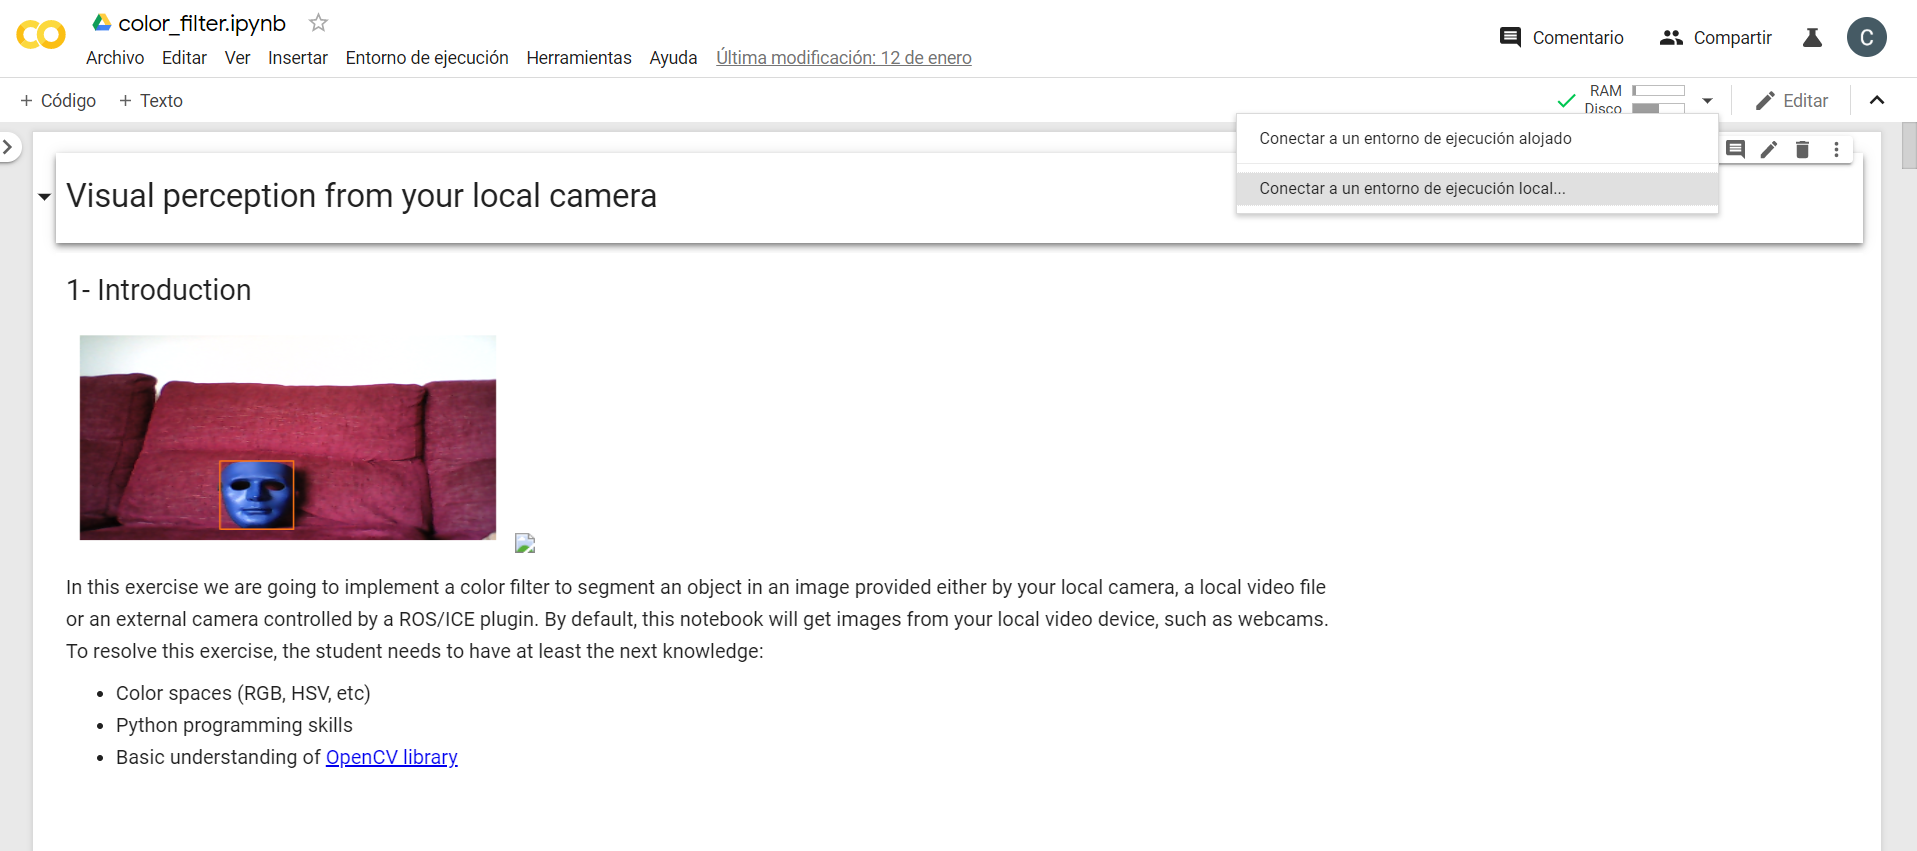
\includegraphics[width=0.99\textwidth,height=7cm]{figures/colab.png}
    \caption{Conexión Local de Colaboratory}
    \label{colab}
\end{figure}
\item [$\rightarrow$]Una plataforma con un gran potencial es la ``\textit{Robot Ignite Academy}\footnote{\url{https://www.robotigniteacademy.com/en/teachers/}} de la empresa The construct \footnote{\url{https://www.theconstructsim.com/}}. Esta plataforma, orientada sobre todo al aprendizaje relacionado con ROS y a las buenas prácticas de trabajo con robots, es una plataforma \textit{on-line} de pago cuyo uso objetivo es principalmente docente para equipos de trabajo o desarrollo en empresas, o para estudiantes de todo el mundo. Busca instruir a los usuarios en entornos prácticos simulados de aprendizaje en forma de cursos de distintos niveles, todos ellos con gran cantidad de detalle para una buena formación. Entre los servicios que oferta, se incluye la construcción desde el principio de un módulo robótico programable cuyo valor docente es importante. Entre sus características destaca que es completamente basado en tecnologías web, y por lo tanto accesible para cualquiera que disponga de un navegador. El rango de robots y escenarios que soporta es limitado (Fig. \ref{theconstruct}).
\begin{figure}[!hbtp]  \centering\noindent
    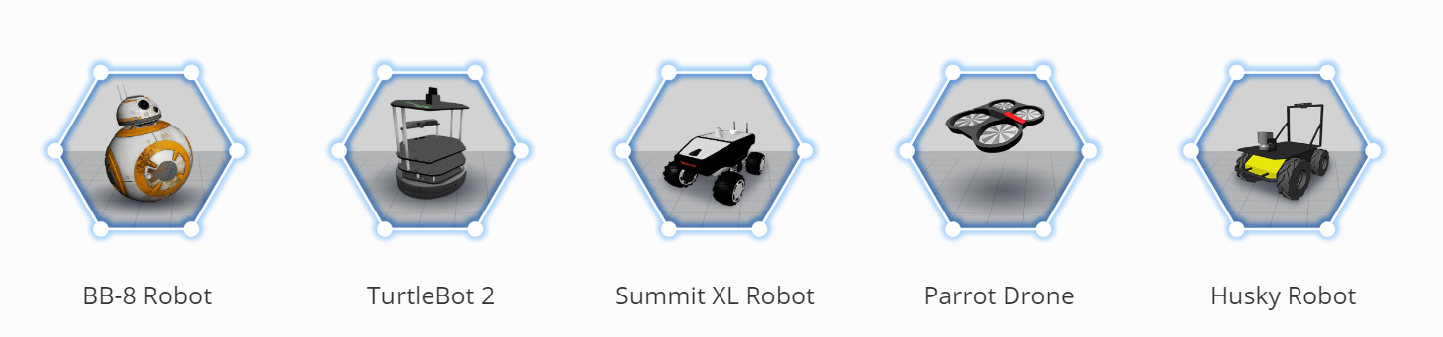
\includegraphics[width=0.95\textwidth]{figures/theconstruct.png}
    \caption{Robots Simulados soportados en Robot Ignite Academy.}
    \label{theconstruct}
\end{figure}
\item [$\rightarrow$] Otro gran ejemplo muy reciente es el entorno \textit{AWS RoboMaker}\footnote{\url{https://aws.amazon.com/es/robomaker/}} de Amazon. Se trata de un servicio que integra herramientas de trabajo con robots, como ROS y entornos de simulación robóticos, que además aprovecha la conectividad en la nube para ofrecer otros servicios, todos ellos propiedad de la empresa, que de nuevo cobra por el servicio que ofrece. Este entorno tiene muchas ventajas en cuanto al proceso de desarrollo e implementación de aplicaciones robóticas inteligentes a gran escala, además de facilitar el proceso de test para probar las aplicaciones que se construyen. Ofrece simulaciones muy realistas y entornos complejos para los robots, de tal manera que se pueden desarrollar comportamientos muy potentes, todo ello en simulación (Fig. \ref{awsrm}). No ofrece soporte para robots reales, aunque sí proporciona un servicio de administración de flotas que simplifica en gran medida el paso de la simulación al sistema físico. Se trata de un entorno web.

\begin{figure}[!hbtp]  \centering\noindent
    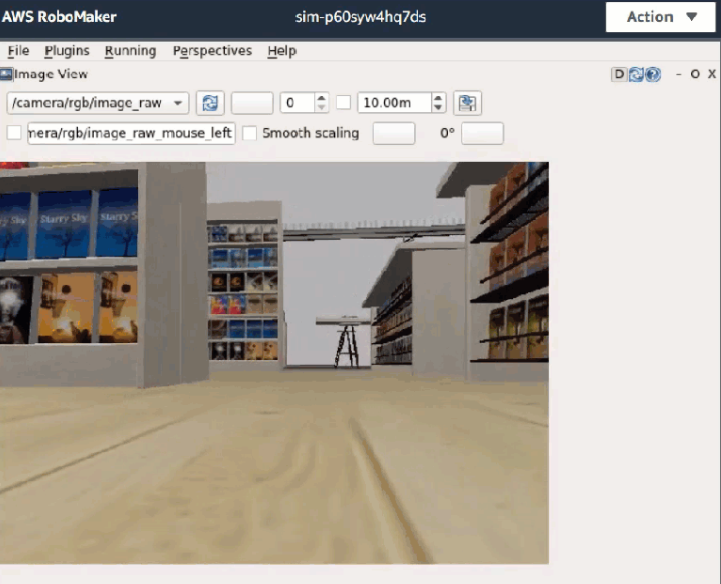
\includegraphics[width=0.8\textwidth]{figures/aws_robomaker.png}
    \caption{Simulación con AWS RoboMaker.}
    \label{awsrm}
\end{figure}

\item [$\rightarrow$] Existen otro tipo de plataformas menos extendidas, en el ámbito nacional e internacional, como JdeRobot\footnote{\url{http://jderobot.org}}, un entorno basado en componentes que se ejecutan como procesos que requiere instalación, y que se especializa en la disposición de todos los elementos necesarios para la fácil construcción de aplicaciones con robots y visión artificial. Si bien soporta tanto robots simulados como reales, este soporte es también limitado (repertorio concreto) y opera sobre las distintas distribuciones del sistema operativo Ubuntu, siendo que en el resto de casos es necesario recurrir a herramientas de virtualización para poder utilizarlo. Este entorno es muy completo y de código abierto, por lo que cualquier usuario puede acceder a él y utilizar toda su funcionalidad. A pesar de su filosofía de \textit{software libre} ofrece calidad profesional (Fig. \ref{jderobot}) a través de la integración de herramientas clásicas de desarrollo robótico como ROS, el simulador Gazebo, las librerías OpenCV y OMPL, etc. Aunque la aplicación es gratuita, requiere amplios conocimiento de programación de robots avanzada para trasladar el código de la simulación al sistema físico.

\begin{figure}[!hbtp]  \centering\noindent
    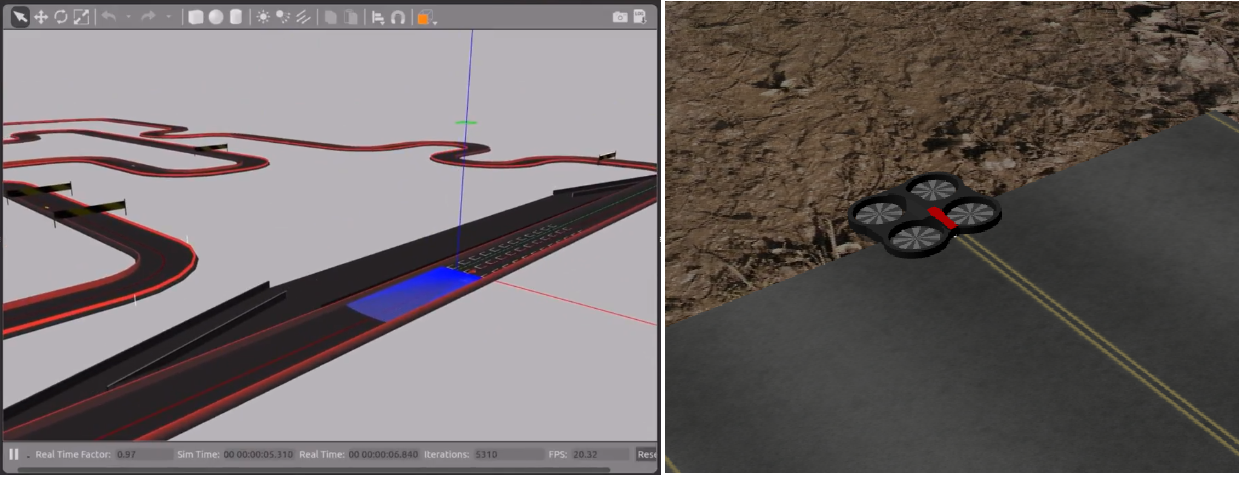
\includegraphics[width=0.8\textwidth]{figures/jderobot_simulation.png}
    \caption{Simulación de aplicación robótica con JdeRobot.}
    \label{jderobot}
\end{figure}

\end{itemize}

Inferimos que hay algo que todos ellos tienen en común: tanto su accesibilidad como su uso son limitados. Las carencias de los entornos actuales radican principalmente en que la mayoría son de pago, muchos de ellos sólo permiten el trabajo en simulación y la totalidad de ellos son incompletos, especialmente en el sentido de que sólo permiten trabajar en un área de la robótica, sólo con un tipo de robot (o una clase) o sólo permiten resolver ciertos problemas para los cuales se prepara un escenario muy controlado. Se observa, aún así, una clara tendencia a ofrecer este tipo de servicio de construcción de aplicaciones como \textit{middleware} a través de la nube para hacerlo más accesible, lo cual supone un punto a tener en cuenta a la hora de evaluar la situación actual y diseñar una nueva idea que colecte y compacte lo mejor de cada uno de los proyectos listados que existen a día de hoy. Es precisamente aquí donde se forma el lugar común entre robótica y tecnologías web, dando paso al entorno que alojará muchas de las aplicaciones robóticas del futuro próximo.

\section{Planteamiento del Problema}

El problema a tratar en esta tesis proviene del análisis de los factores que hacen distinto el desarrollo y el aprendizaje en este campo, y de cómo estos factores suponen un obstáculo, y en ocasiones incluso un impedimento, a la hora de realizar un proyecto específico. En este punto cabe preguntarse por qué no existen infinidad de plataformas y herramientas en la nube dotadas de aquellas características deseables para el aprendizaje y la investigación en el ámbito de los robots. 

Por un lado está el ya mencionado factor económico. Si nos paramos a pensar en el motivo por el cual las plataformas existentes se plantean como un servicio por el que hay que pagar caemos en la cuenta de que, aunque haya una parte debida al coste de desarrollo de dicha plataforma y al valor estratégico del producto que cubre una necesidad global en auge, principalmente se debe al consumo de recursos asociado a cualquier proyecto robótico en cualquier ámbito. Trabajar en robótica es sinónimo de disponer de recursos. Es bien sabido que el \textit{hardware} es caro y frágil, que la implementación tanto del sistema físico como de la lógica programada es temporalmente costosa y que incluso con la ausencia de sistemas reales, el coste computacional es enormemente elevado debido a que están involucrados programas exigentes como los simuladores robóticos y también dada la necesidad de un control estricto y veloz de todos los submódulos que componen un proyecto robótico, cada uno de ellos encargado de una tarea que requiere de más y más capacidad para realizar operaciones por unidad temporal. El primer obstáculo encontrado durante el análisis fue precisamente que \textbf{el consumo de recursos genera costes}, y que estos costes son elevados.

Por otro lado, en mi opinión, aprender robótica exige robots. Ya no sólo desde el punto de vista económico sino también desde el logístico, es complicado crear un servicio que disponga de tantos robots como usuarios y que pueda acarrear con los costes derivados de su uso por todo el que lo requiera. Aún pudiendo afrontarlos, construir un sistema que permitiese al usuario, sea estudiante, investigador o simple curioso, evaluar el código de su aplicación sobre un elemento \textit{hardware} remoto y acceder a los resultados en tiempo de ejecución sería una ardua tarea. Por tanto, el análisis realizado destacó que \textbf{desarrollar aplicaciones robóticas requiere disponer de realimentación, visual y paramétrica, en tiempo real}, sólo alcanzable a través de la observación de sistemas electro-mecánicos reales.

Por último, generalmente se desarrolla una gran cantidad de herramientas y plataformas que soportan sistemas específicos, es decir, de funcionalidad acotada. Esto supone un problema para el usuario medio ya que, normalmente, \textbf{carece de \textit{hardware} específico. Sin embargo, sí que tiene acceso a sistemas más básicos}. Esta circunstancia resultó ser la tercera clave extraída del estudio previo.

Así las cosas, la conclusión a la que se llegó es que no existen actualmente herramientas que simplifiquen el uso docente y de investigación de la robótica. Con todo lo anterior y sin perder de vista la idea de ``Acercar la robótica a la gente'', el problema radica precisamente en sortear esos obstáculos.
